\documentclass[oneside, abstracton, titlepage]{scrartcl}

\usepackage[left=2.5cm,right=2.6cm,top=3cm,bottom=3cm]{geometry}
\usepackage[utf8]{inputenc}
\usepackage[intlimits]{amsmath}
\usepackage{amssymb}
\usepackage{color}
\usepackage{subcaption}
\usepackage[version=4]{mhchem}

\usepackage{graphicx}

\begin{document}

\section{Example: Regulation of gene expression}\label{sec:generegulation}

To demonstrate our method we estimate a gene-regulatory network from data. The data is time-series of molecule-concentrations obtained from law of mass action (LMA) equations with additive gaussian noise.

Let A, B and C be the three species of proteins. Each of them is translated from its according mRNA molecule. Each mRNA molecule is transcribed from its according DNA. The proteins and mRNA molecules decay over time. For each species one can formulate the following basic reactions
\begin{align*}
    \ce{ DNA_i } & \ce{ -> DNA_i + mRNA_i } &\text{(transcription)} \\
    \ce{ mRNA_i } & \ce{ -> mRNA_i + Protein_i } &\text{(translation)} \\
    \ce{ mRNA_i } & \ce{ -> } \emptyset &\text{(decay of mRNA)} \\
    \ce{ Protein_i } & \ce{ -> } \emptyset &\text{(decay of Protein)}
\end{align*}

A, B and C regulate each other in a negative way, by hindering the transcription process. In the LMA model we account for this by a reaction. A repression of species $j$ by species $i$ is modeled as
\begin{equation*}
    \ce{ Protein_i + mRNA_j -> Protein_i } \quad \text{(regulation by repression)}
\end{equation*}

In our example A proteins regulate the mRNA$_\mathrm{B}$ molecules, B proteins regulate the mRNA$_\mathrm{A}$ molecules and C proteins regulate the mRNA$_\mathrm{A}$ molecules. The network of all species and reactions is depicted in figure ???????. This will serve as our reference model to generate the time-series of concentrations.
\begin{figure}
    \centering
    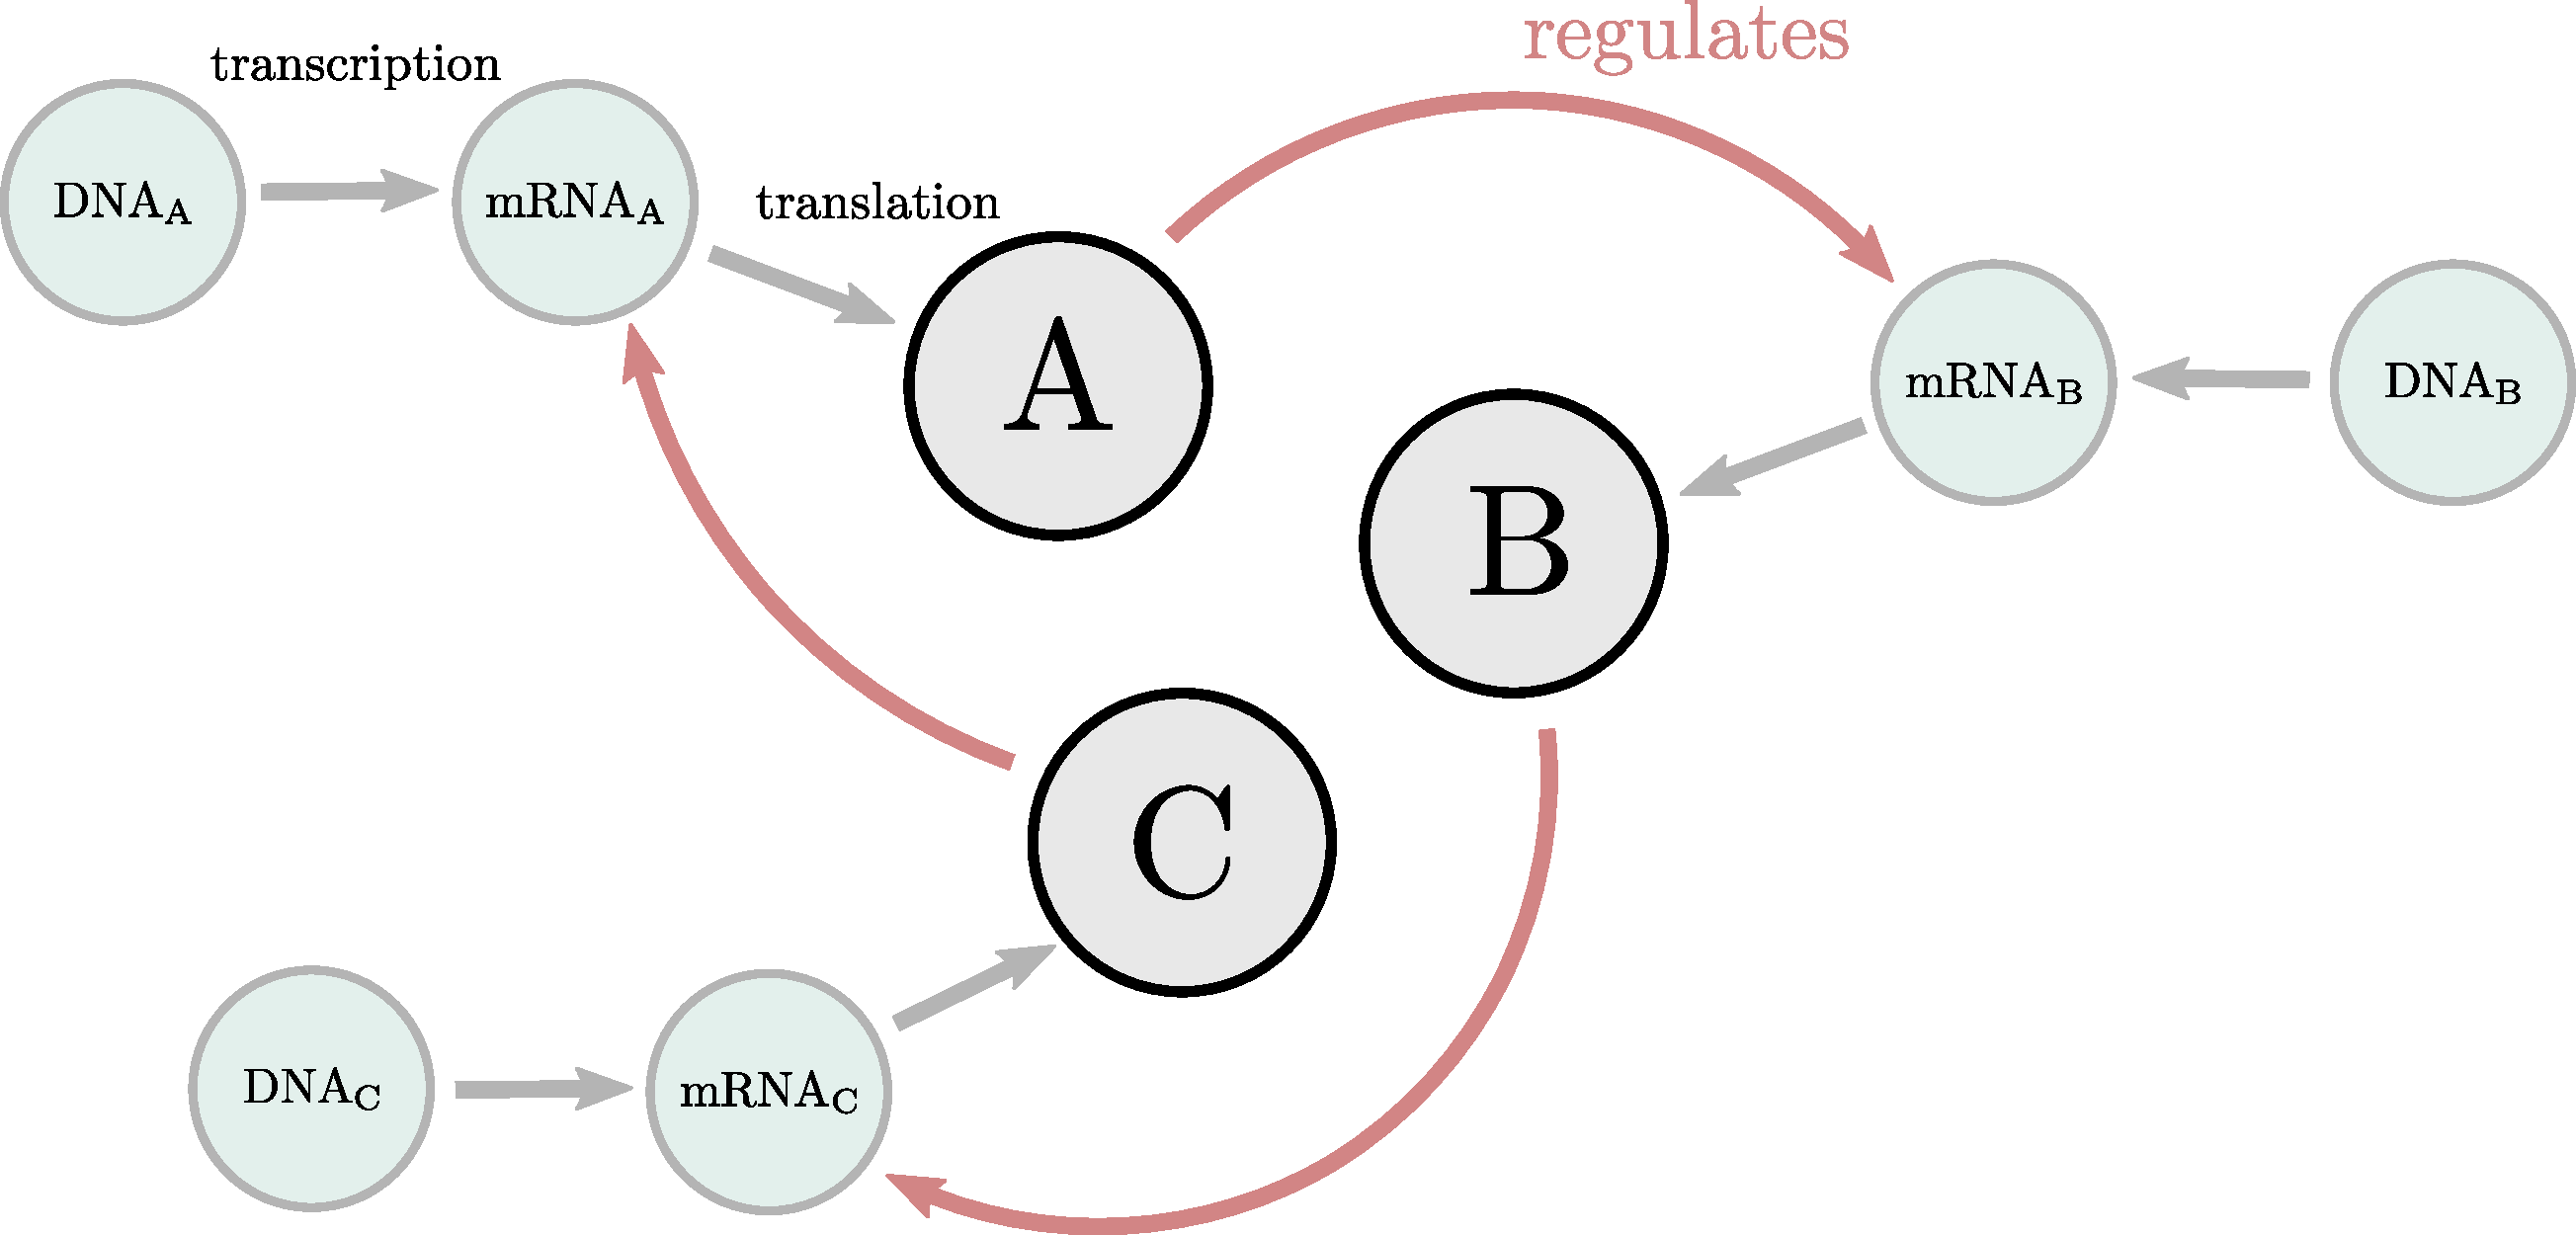
\includegraphics[width=.5\textwidth]{./figures_tex/gene_regulation_full.pdf}
    \caption{The regulation network example described in Section \ref{sec:generegulation}. Each circle is a species, each arrow corresponds to one reaction. The red arrows describe the reference regulatory network which generates our data.}
    \label{fig:network}
\end{figure}


\end{document}
